%preamble - package inclusion and set up
\documentclass[12pt,twoside,a4paper,english]{report} %normalt 12pt!!!!
% Select encoding of your inputs
\usepackage[utf8]{inputenc}
% Make latex understand and use the typographic
% rules of the language used in the document.
%\usepackage[danish]{babel}
\usepackage[english]{babel}

% Use the vector font Latin Modern which is going
% to be the default font in latex in the future.
\usepackage{lmodern}
%\usepackage{mathptmx}

% Choose the font encoding
\usepackage[T1]{fontenc}

% Use color in tables
\usepackage[table]{xcolor}
\usepackage{pbox}
\usepackage{tabularx}
\usepackage{array}
\usepackage{multirow}

% Load a colour package
\usepackage{xcolor}
\definecolor{aaublue}{RGB}{33,26,82}  %<--define aaublue
\definecolor{white}{RGB}{255,255,255} %<--define white

% ref stuffz			original position
%\usepackage{cleveref}

% The standard graphics inclusion package
\usepackage{graphicx}

\makeatletter
  \g@addto@macro\@floatboxreset\centering %<--centering all figures
\makeatother

\usepackage{adjustbox}

% Set up how figure and table captions are displayed

\usepackage{float}
\restylefloat{figure}
\usepackage{caption}
\usepackage{subfigure}
\usepackage[subfigure]{tocloft}
\captionsetup
{
  %justification = centering,    %<--centering caption with multiple lines
  %justification = raggedright,  %<-- right alings caption with multiple lines
  justification = justified,  %<-- justify alings (make left and right side equal) caption with multiple lines
  font          = footnotesize, %<--set font size to footnotesize
  labelfont     = bf            %<--bold label (e.g., Figure 3.2) font
}
\captionsetup[subfigure]
{
  justification = centering, %<--centering subfigure caption text
  singlelinecheck=false,
  font = footnotesize        %<--font size for subfigures
} 

% Enable row combination in tables
\usepackage{multirow}

% Make space between table lines and text
\renewcommand{\arraystretch}{1.5}

% Enable commands like \st (strike out) and \hl (high light)
\usepackage{soul}

% Make the standard latex tables look so much better
\usepackage{array,booktabs}

% Enable the use of frames around, e.g., theorems
% The framed package is used in the example environment
\usepackage{framed}
\usepackage{colortbl}
\usepackage{longtable}
\usepackage{xcolor}
\usepackage{textcomp}
\usepackage{indentfirst}
\setlength{\parindent}{1.5cm}
%-------MATHEMATICS---------------------------------
% Defines new environments such as equation,
% align and split 
\usepackage{amsmath}
\usepackage{relsize}
% Adds new math symbols
\usepackage{amssymb}
% Use theorems in your document
% The ntheorem package is also used for the example environment
% When using thmmarks, amsmath must be an option as well. Otherwise \eqref doesn't work anymore.
\usepackage[framed,amsmath,thmmarks]{ntheorem}
\usepackage{xifthen}%<--enables ifthenelse which is used in macros

\usepackage{siunitx} 
\sisetup{decimalsymbol=period}%<--\num{} will swich commas with periods
\sisetup{detect-weight}
%---------------------------------------------------

%-------PAGE LAYOUT---------------------------------
% Change margins, papersize, etc of the document
\usepackage[
  left=25mm,% left margin on an odd page %tidligere 25mm for baade right og left
  right=25mm,% right margin on an odd page
  top=35mm,
  ]{geometry}
  
% Modify how \chapter, \section, etc. look
% The titlesec package is very configureable
\usepackage{titlesec}
\makeatletter
\def\ttl@mkchap@i#1#2#3#4#5#6#7{%
    \ttl@assign\@tempskipa#3\relax\beforetitleunit
    \vspace{\@tempskipa}%<<<<<< REMOVE THE * AFTER \vspace
    \global\@afterindenttrue
    \ifcase#5 \global\@afterindentfalse\fi
    \ttl@assign\@tempskipb#4\relax\aftertitleunit
    \ttl@topmode{\@tempskipb}{%
        \ttl@select{#6}{#1}{#2}{#7}}%
    \ttl@finmarks  % Outside the box!
    \@ifundefined{ttlp@#6}{}{\ttlp@write{#6}}}
\makeatother

\titlespacing{\chapter}{0pt}{0pt}{10pt}
\titlespacing{\section}{0pt}{0pt}{-5pt}
\titlespacing{\subsection}{0pt}{8pt}{-5pt}
\titlespacing{\subsubsection}{0pt}{6pt}{-10pt}

\titleformat*{\section}{\normalfont\Large\bfseries\color{aaublue}}
\titleformat*{\subsection}{\normalfont\large\bfseries\color{aaublue}}
\titleformat*{\subsubsection}{\normalfont\normalsize\bfseries\color{aaublue}}

\usepackage{titlesec, blindtext, color}
%\color{gray75}{gray}{0.75}
\newcommand{\hsp}{\hspace{20pt}}
\titleformat{\chapter}[hang]{\Huge\bfseries}{\thechapter\hsp\textcolor{aaublue}{|}\hsp}{0pt}{\Huge\bfseries}

% Change the headers and footers
\usepackage{fancyhdr}
\setlength{\headheight}{15pt}
\pagestyle{fancy}
\fancyhf{} %delete everything
\renewcommand{\headrulewidth}{0pt} %remove the horizontal line in the header
\fancyhead[RO,LE]{\color{aaublue}\small\nouppercase\leftmark} %even page - chapter title
\fancyhead[LO]{}
\fancyhead[RE]{} 
\fancyhead[CE]{}
\fancyhead[CO]{}
\fancyfoot[RE,LO]{\thepage}
\fancyfoot[LE,RO]{} %page number on all pages
\fancyfoot[CE,CO]{}

% change first page of all chapters header and footer to fancy style
\makeatletter
\let\ps@plain\ps@fancy
\makeatother

% Do not stretch the content of a page. Instead,
% insert white space at the bottom of the page
\raggedbottom

% Enable arithmetics with length. Useful when typesetting the layout.
\usepackage{calc}
%---------------------------------------------------

\usepackage{appendix}

%-------BIBLIOGRAPHY--------------------------------
%setting references (using numbers) and supporting i.a. Chicargo-style:
\usepackage{etex}
\usepackage{etoolbox}
\usepackage{keyval}
\usepackage{ifthen}
\usepackage{url}
\usepackage{csquotes}
\usepackage[backend=bibtex, isbn=false, url=false, eprint=false, doi=false, style=numeric, sorting=none]{biblatex}
\addbibresource{setup/bibliography.bib}
%---------------------------------------------------

%-------MISC----------------------------------------
%%% Enables the use FiXme refferences. Syntax: \fxnote{...} %%%
\usepackage[footnote, draft, english, silent, nomargin]{fixme}		%!!!! DRAFT OR FINAL?!?!?!?!11!! change later!	
%With "final" instead of "draft" an error will ocure for every FiXme under compilation.

%%% allows use of lorem ipsum (generate i.e. pagagraph 1 to 5 with \lipsum[1-5]) %%%
\usepackage{lipsum}

%%% Enables figures with text wrapped tightly around it %%%
\usepackage{wrapfig}

%%% Section debth included in table of contents (1 = down to sections) %%%
\setcounter{tocdepth}{1}

%%% Section debth for numbers (1 = down to sections) %%%
\setcounter{secnumdepth}{2}

\usepackage{tocloft}
\setlength{\cftbeforetoctitleskip}{0 cm}
\renewcommand{\cftpartpresnum}{Part~}
\let\cftoldpartfont\cftpartfont
\renewcommand{\cftpartfont}{\cftoldpartfont\cftpartpresnum}
%---------------------------------------------------

%-------DANSK SPROG---------------------------------

%\addto\captionsdanish{%
%	\renewcommand{\figurename}{figur}%
%	\let\figureautorefname\figurename%
%	\renewcommand{\tablename}{tabel}%
%	\let\tableautorefname\tablename%
%%	\renewcommand{\equationname}{ligning}%
%%	\let\equationautorefname\equationname%
%	\renewcommand{\chaptername}{Kapitel}%
%	\let\chapterautorefname\chaptername%
%	\renewcommand{\partname}{Del}%
%	\let\partautorefname\partname%
%	\renewcommand{\sectionname}{afsnit}%
%	\let\sectionautorefname\sectionname%
%%	\renewcommand{\thesubsection}{underafsnit}%
%%	\let\subsectionautorefname\thesubsection%
%	\renewcommand{\pagename}{side}%
%	\let\pageautorefname\pagename%
%}

%-------HYPERLINKS----------------------------------
% Enable hyperlinks and insert info into the pdf
% file. Hypperref should be loaded as one of the 
% last packages
\usepackage{nameref}
\usepackage{hyperref}
\usepackage{bookmark}
\hypersetup{%
	%pdfpagelabels=true,%
	plainpages=false,%
	pdfauthor={Author(s)},%
	pdftitle={Title},%
	pdfsubject={Subject},%
	bookmarksnumbered=true,%
	colorlinks,%
	citecolor=aaublue,%
	filecolor=aaublue,%
	linkcolor=aaublue,% you should probably change this to black before printing
	urlcolor=aaublue,%
	pdfstartview=FitH%
}

% ref stuffz		new position
\usepackage{cleveref}

\crefname{appsec}{bilag}{bilag}
%---------------------------------------------------



% remove all indentations
\setlength\parindent{0pt}
\parskip 5mm
\usepackage{verbatim}

\definecolor{Gra}{RGB}{230,230,230}

%creates a nice-looking C#-text
\newcommand{\CC}{C\nolinebreak\hspace{-.05em}\raisebox{.3ex}{\scriptsize\text \#} }

%enables multi column lists
\usepackage{multicol}

%enables code-examples
\usepackage{listings}

\definecolor{coolblue}{RGB}{32,95,128}
\definecolor{mygreen}{rgb}{0,0.6,0}
\definecolor{mygray}{rgb}{0.5,0.5,0.5}
\definecolor{mymauve}{rgb}{0.58,0,0.82}
\usepackage{textcomp}
\definecolor{listinggray}{gray}{0.9}
\definecolor{lbcolor}{rgb}{0.9,0.9,0.9}

%for c code
\lstdefinestyle{cstyle}{
  backgroundcolor=\color{lbcolor},
	tabsize=4,
	rulecolor=,
	language=C,
  basicstyle=\scriptsize,
  upquote=true,
  aboveskip={1.5\baselineskip},
  columns=fixed,
  showstringspaces=false,
  extendedchars=true,
  breaklines=true,
  prebreak = \raisebox{0ex}[0ex][0ex]{\ensuremath{\hookleftarrow}},
  frame=single,
  showtabs=false,
  numbers=left,
  captionpos=b,
  numbersep=5pt,
  numberstyle=\tiny\color{mygray},
  showspaces=false,
  showstringspaces=false,
  identifierstyle=\ttfamily,
  keywordstyle=\color[rgb]{0,0,1},
  commentstyle=\color[rgb]{0.133,0.545,0.133},
  stringstyle=\color[rgb]{0.627,0.126,0.941},
}
%for python code
\lstdefinestyle{pythonstyle}{
    backgroundcolor=\color{lbcolor},
    tabsize=4,
    rulecolor=,
    language=python,
    basicstyle=\scriptsize,
    upquote=true,
    aboveskip={1.5\baselineskip},
    columns=fixed,
    showstringspaces=false,
    extendedchars=true,
    breaklines=true,
    prebreak = \raisebox{0ex}[0ex][0ex]{\ensuremath{\hookleftarrow}},
    frame=single,
    showtabs=false,
    numbers=left,
    captionpos=b,
    numbersep=5pt,
    numberstyle=\tiny\color{mygray},
    showspaces=false,
    showstringspaces=false,
    identifierstyle=\ttfamily,
    keywordstyle=\color[rgb]{0,0,1},
    commentstyle=\color[rgb]{0.133,0.545,0.133},
    stringstyle=\color[rgb]{0.627,0.126,0.941},
}
%for matlab code
\lstdefinestyle{matlabstyle}{
    backgroundcolor=\color{lbcolor},
    tabsize=4,
    rulecolor=,
    language=Matlab,
    basicstyle=\scriptsize,
    upquote=true,
    aboveskip={1.5\baselineskip},
    columns=fixed,
    showstringspaces=false,
    extendedchars=true,
    breaklines=true,
    prebreak = \raisebox{0ex}[0ex][0ex]{\ensuremath{\hookleftarrow}},
    frame=single,
    showtabs=false,
    numbers=left,
    captionpos=b,
    numbersep=5pt,
    numberstyle=\tiny\color{mygray},
    showspaces=false,
    showstringspaces=false,
    identifierstyle=\ttfamily,
    keywordstyle=\color[rgb]{0,0,1},
    commentstyle=\color[rgb]{0.133,0.545,0.133},
    stringstyle=\color[rgb]{0.627,0.126,0.941},   
}

%for java code
\lstdefinestyle{javastyle}{
	backgroundcolor=\color{lbcolor},
	tabsize=4,
	rulecolor=,
	language=Java,
	basicstyle=\scriptsize,
	upquote=true,
	aboveskip={1.5\baselineskip},
	columns=fixed,
	showstringspaces=false,
	extendedchars=true,
	breaklines=true,
	prebreak = \raisebox{0ex}[0ex][0ex]{\ensuremath{\hookleftarrow}},
	frame=single,
	showtabs=false,
	numbers=left,
	captionpos=b,
	numbersep=5pt,
	numberstyle=\tiny\color{mygray},
	showspaces=false,
	showstringspaces=false,
	identifierstyle=\ttfamily,
	keywordstyle=\color[rgb]{0,0,1},
	commentstyle=\color[rgb]{0.133,0.545,0.133},
	stringstyle=\color[rgb]{0.627,0.126,0.941},
}

%for inline c, syntax: \cline{ codeHere(); }
\lstdefinestyle{cinline}{
    style=cstyle,
    basicstyle=\small,
}
\newcommand\inlinec[1]{ \lstinline[style=cinline]{#1} }

%for inline python, syntax: \pythonline{ codeHere(); }
\lstdefinestyle{pythoninline}{
    style=pythonstyle,
    basicstyle=\small,
}
\newcommand\inlinepython[1]{ \lstinline[style=pythoninline]{#1} }

%for inline matlab, syntax: \matlabline{ codeHere(); }
\lstdefinestyle{matlabinline}{
    style=matlabstyle,
    basicstyle=\small,
}
\newcommand\inlinematlab[1]{ \lstinline[style=matlabinline]{#1} }

\usepackage{enumitem}
%\usepackage[citestyle=authoryear,natbib=true]{biblatex}

% Figures - TIKZ
\usepackage{tikz}
\usepackage[americanresistors,americaninductors,americancurrents, americanvoltages]{circuitikz}

% Wall of text logo
\newcommand{\walloftextalert}[0]{\includegraphics[width=\textwidth]{walloftext.png}}

\usepackage{pdfpages}
\usepackage{lastpage}
\usepackage{epstopdf}

\setlength{\headheight}{21pt}

\hfuzz=\maxdimen
\tolerance = 10000
\hbadness  = 10000

\usepackage{siunitx}
\graphicspath{{./figures/}}

%macros - please read this file
%Macro for 'where'-enviroment was improved by Andrea and Niels :-)

%-----------UNITS-------------------------------------------
\newcommand{\unit}[1]{&& \left[\si{#1}\right]}
%
%\newcommand{\unit}[1]{[\si{#1}]}            %<<| Use these if you want equations to be
%\newcommand{\eq}[2]{&&\si{#1} &= \si{#2}&&} %<<| centered.. .. will appear scrambled
%                                            %  | from one equation to the next though..
%                                            %  | and does not work with long equations.. :/
%
%-----------------------------------------------------------

%-----------WHERE ENVIRONMENT-------------------------------
\newenvironment{where}{\leavevmode{\parindent=1em\indent} Where:\\}{}
\newcommand{\va}[3]
{
  \begin{tabular}{p{20pt} p{40pt} p{290pt} l}
    & { $#1$ } & { #2 } & \ifthenelse{\isempty{ #3 }}  {}  {[{\si{#3}}]} \\
  \end{tabular}\\
}
%-----------------------------------------------------------

%-----------TikZ SETTINGS-----------------------------------
\tikzset{
  block/.style    = {draw, thick, rectangle,
                     minimum height = 2.1em,
                     minimum width = 1.7em},
  sum/.style      = {draw, circle, inner sep=3pt} %<--Adder
}
%-----------------------------------------------------------


%-----------Fanzy reference SETTINGS------------------------
%Figure references:
\newcommand{\figref}[1]{figure \ref{#1}}

%Figure references after full stop/period:
\newcommand{\Figref}[1]{Figure \ref{#1}}

%Table references:
\newcommand{\tabref}[1]{table \ref{#1}}

%Table references after full stop/period:
\newcommand{\Tabref}[1]{Table \ref{#1}}

%Section references:
\newcommand{\secref}[1]{section \ref{#1}} % on page \pageref{#1}}

%Section references:
\newcommand{\Secref}[1]{Section \ref{#1}} % on page \pageref{#1}}

%Subsection references:
\renewcommand{\subref}[1]{section \ref{#1}} % on page \pageref{#1}}

%Subsection references:
\renewcommand{\Subref}[1]{Section \ref{#1}} % on page \pageref{#1}}

%Appendix references:
\newcommand{\appref}[1]{appendix \ref{#1}} % on page \pageref{#1}}

%Appendix references:
\newcommand{\Appref}[1]{Appendix \ref{#1}} % on page \pageref{#1}}

%chapter references: 
\newcommand{\chapref}[1]{chapter \ref{#1}} % on page \pageref{#1}}

%chapter references: 
\newcommand{\Chapref}[1]{Chapter \ref{#1}} % on page \pageref{#1}}

%Units:
%\newcommand{\unit}[1]{&& \left[\si{#1}\right]}

%Text:
\newcommand{\tx}[1]{\text{#1}}

%Equation references:
%1 equation:
\renewcommand{\eqref}[1]{equation (\ref{#1})}

%-----------------------------------------------------------





\begin{document}       % TIP: If you are using TeXstudio you can open
%\tableofcontents      %      the file by Ctrl+LeftClick on setup/macros.tex
%\pagebreak             %      If the file doesn't exist, you will be asked
					   %      weather or not you want to create it.
%\begin{center}
%	\vspace{5cm}
%	\Huge{Worksheets}
%\end{center}
%\clearpage

%||||||||||||||||||||||||||||||||||||||||||||||||||||||||||||||||
%|||||||                 Example Inputs                  ||||||||
%||||||||||||||||||||||||||||||||||||||||||||||||||||||||||||||||
%|||||||                                                 ||||||||
%			 \input{chapters/aFigureSample.tex}			 %|||||||
%			 \input{chapters/bTableSample.tex} 		     %|||||||
%			 \input{chapters/cEquationSample.tex}		 %|||||||
%			 \input{chapters/dTikzSample.tex}            %|||||||
%			 \input{chapters/eCodeSample.tex}            %|||||||
%|||||||                                                 ||||||||
%||||||||||||||||||||||||||||||||||||||||||||||||||||||||||||||||
%||||||||||||||||||||||||||||||||||||||||||||||||||||||||||||||||


%%% Prereport %%%
		\setlength\cftaftertoctitleskip{2pt}
		\setlength\cftafterloftitleskip{6pt}
		\setlength\cftafterlottitleskip{6pt}
%\selectlanguage{danish}
%\title{Something about the coolest preprocessing methods and nice results for IDP study}

%%% Frontmatter Settings %%%
		\pagestyle{empty} %disable headers and footers
		\pagenumbering{roman} %use roman page numbering in the frontmatter I II...
	%	\fancyfoot[RE,LO]{18??} %page number on all pages
		\fancyfoot[LE,RO]{\thepage}
		\fancyhead[LE,LO,RE,RO]{}

%%% Introductory Formalities %%%
%\includepdf[pages={1}]{formalities/frontpage.tex}
			\clearpage
\thispagestyle{empty}

\begin{figure}[H]
	\raggedleft
	
\includegraphics[width=0.2\textwidth]{figures/aaulogo-en.png}
\end{figure} 

\vspace{5 cm}

\begin{center}
	\begin{Huge}
		\textbf{Evaluation of Electrotactile Feedback Schemes in a
			Closed-Loop Myoelectric Prosthesis}\\
		\vspace{5 mm}
		Master Thesis \\
		Biomedical Engineering \& Informatics - Spring $2019$\\
		\vspace{3 mm}
	\end{Huge}
	{\Large Project group: $19$gr$10407$} \\
	\vspace{1cm}
	\large{Christian Korfitz Mortensen, Martin Alexander Garenfeld}
\end{center}
\vspace*{\fill}

\begin{center}
	\line(1,0){400}
\end{center}

%\newpage
%
%\large{\textbf{Project period:}\\
%P7, Autumn 2017\\
%01/08/2017 - 20/12/2017\\
%
%\textbf{Project group:}\\
%17gr7404\\} %\fxnote{Input group number}
%
%
%\begin{center}
%	\Large{\textbf{Collaborators:}\\
%		\vspace{1.5cm}
%	\rule{10cm}{1pt}\\
%	Irene Uriarte \\
%	
%	\rule{10cm}{1pt}\\
%	Martin Alexander Garenfeld \\
%	
%	\rule{10cm}{1pt}\\
%	Oliver Thomsen Damsgaard \\
%	
%	\rule{10cm}{1pt}\\
%	Simon Bruun \\}
%\end{center}
%
%
%
%\large{\textbf{Supervisors:}\\
%Strahinja Dosen \\
%Jakob Lund Dideriksen \\
%Lotte N.S. Andreasen Struijk} \\
%\\
\newpage
			% <--- the frontpage
			\pagestyle{fancy}
%{\small
\strut\vfill % push the content to the bottom of the page
\noindent Copyright \copyright{} Aalborg University 2015\par
\vspace{0.2cm}

\noindent This report is compiled in \LaTeX, originally developed by Leslie Lamport, based on Donald Knuth's \TeX. The main text is written in \emph{Latin Modern} pt 12, designed by Bogusław Jackowski and Janusz M. Nowacki. 
%The document is compiled via the website \url{www.overleaf.com}, an online collaborative based \LaTeX-editor with instant preview, which enables multiple persons to edit the document simultaneously.
Flowcharts and diagrams are made using Microsoft Visio. 
\clearpage
%			%\begin{document} 
\thispagestyle{empty}
\begin{titlepage}
	\begin{nopagebreak}
		{\samepage 
			
			\begin{tabular}{r}
				\parbox{\textwidth}{  \raisebox{-15mm}{
\includegraphics[height=3cm]{figures/aaulogo-en.png}}
					\hfill \hspace{2cm} \parbox{8cm}{\begin{tabular}{l} %4.90
							{\small \textbf{\textcolor{aaublue}{{3\textsuperscript{rd} Semester, Project}}}}\\
							{\small \textbf{\textcolor{aaublue}{School of Medicine and Health}}}\\
							%{\small \textbf{\textcolor{aaublue}{Communication Technologies}}}\\ 
							{\small \textbf{\textcolor{aaublue}{Biomedical Engineering and Informatics}}}\\
							{\small \textcolor{aaublue}{Fredrik Bajers Vej 7A}} \\
							{\small \textcolor{aaublue}{9220 Aalborg}} \\
							%{\small \textcolor{aaublue}{\emph{http://www.sict.aau.dk/electronics-and-it}}}
				\end{tabular}}}
			\end{tabular}
			
			\begin{tabular}{cc}
				\parbox{7cm}{
					
					\textbf{Title:}
					
					Does Task-related FMRI Preprocessing Need a FIX? \\ 
					
					\textbf{Theme:}
					
					\small{
						Applied Biomedical Engineering and Informatics\\
					}
					
					
					\parbox{8cm}{
						
						
						\textbf{Project period:}\\
						P3, Fall 2018\\
						01/09/2018 - 20/12/2018\\
						
						\textbf{Project group:}\\
						18gr9411\\ %\fxnote{Input group number}
						
						\textbf{Participants:}\\
						Christian Korfitz Mortensen\\
						Martin Alexander Garenfeld\\
						
						
						
						\textbf{Supervisors:}\\
						Robert Coghill\\
						Marie-Eve Hoeppli\\
						Carsten Dahl Mørch\\
						
					}\\
					\\
					\\
					\textbf{Pages:} 83\\
					\textbf{Appendix:} 13 \\
					%\textbf{Ekstra:} For projektkode: Se forord\\ %eks. en CD eller USB
					\textbf{Handed in:} 19/12/2018\\
					\\
					\textit{The content of this report is freely available, but publication (with reference) may only be done with
						agreement with the authors.}
					\vfill } &
				\parbox{7cm}{
					\vspace{-.55cm}
					\hfill
					\begin{tabular}{l}
						{\textbf{Abstract:}} \\
						\fbox{
							\parbox{8.5cm}{\bigskip
								{\vfill{\small The implementation of intuitive and meaningful proprioceptive feedback of myoelectric prosthetic states is an important aspect in enhancing embodiment and user satisfaction, hence lowering the demand for visual attention for prosthetic control in everyday tasks. Therefore, two different configurations for conveying position state information of wrist rotation and hand aperture through electrotactile stimulation were developed and evaluated in a simulated closed-loop prosthesis. A spatially-based configuration was made conveying information by changing the activation of pads in an electrode array placed circumferentially around the non-dominant arm. The other scheme was amplitude-based and used various levels of amplitude from specific electrode pads to convey information of the position state of the prosthesis. 14 able-bodied subjects were evaluated through a Fitts' Law inspired target reaching test following a minimal training session.
The amplitude-based and spatially-based configurations yielded mean completion rates of 93 \% $\boldsymbol{\pm}$ 6 \% and 87 \% $\boldsymbol{\pm}$ 11 \%, respectively. The amplitude feedback configuration yielded a slightly higher completion rate (p = 0.044) than the spatially-based and was also preferred by 64 \% of the subjects. However, with such high completion rates both schemes can be regarded intuitive and was subjectively reported to be useful and easily comprehensible. This manifests that both developed feedback configurations allow subjects to perceive two feedback variables at the same time, despite being implemented in a compact stimulation interface.
										\bigskip}}
						}}
				\end{tabular}}
		\end{tabular}} %\vspace{1cm}
		
		
		%\centering
		%\textit{Offentliggørelse af rapportens indhold, med kildeangivelse, må kun ske efter aftale med forfatterne.}\\
		
	\end{nopagebreak}
\end{titlepage}
%\end{document} 			 % <--- the titlesheet - contains the synopsis!!
%%% Preface %%%
			\cleardoublepage
			
%			The implementation of intuitive and meaningful proprioceptive feedback of myoelectric prosthetic states is an important aspect in enhancing embodiment and user satisfaction, hence lowering the demand for visual attention for prosthetic control in everyday tasks. Therefore, two different configurations for conveying position state information of wrist rotation and hand aperture through electrotactile stimulation were developed and evaluated in a simulated closed-loop prosthesis. A spatially-based configuration was made conveying information by changing the activation of pads in an electrode array placed circumferentially around the non-dominant arm. The other scheme was amplitude-based and used various levels of amplitude from specific electrode pads to convey information of the position state of the prosthesis. 14 able-bodied subjects were evaluated through a Fitts' Law inspired target reaching test following a minimal training session.
The amplitude-based and spatially-based configurations yielded mean completion rates of 93 \% $\boldsymbol{\pm}$ 6 \% and 87 \% $\boldsymbol{\pm}$ 11 \%, respectively. The amplitude feedback configuration yielded a slightly higher completion rate (p = 0.044) than the spatially-based and was also preferred by 64 \% of the subjects. However, with such high completion rates both schemes can be regarded intuitive and was subjectively reported to be useful and easily comprehensible. This manifests that both developed feedback configurations allow subjects to perceive two feedback variables at the same time, despite being implemented in a compact stimulation interface.			 % <--- this is the abstract!!
\clearpage
	%		\chapter*{Preface}				% <--- the preface
%
%\input{contents/bBackground/title.tex}
\clearpage
			\pdfbookmark[0]{Table of Contents}{label: tableOfCentents}
			\tableofcontents
			\cleardoublepage


%%% Mainmatter Settings %%%
\pagenumbering{arabic} %use arabic page numbering in the mainmatter
\fancyhf{}
\fancyfoot[C]{\thepage} %\text{ of} \pageref{LastPage}			% ADD LABLE{LASTPAGE} TO LAST PAGE !!
\fancyfoot[RE,LO]{19gr10407}																								   %
\fancyhead[RE,LO]{}																												%% } consider fancyfoots
\fancyhead[RE,LO]{\color{aaublue}\small\nouppercase\leftmark} %even page - chapter title %
\pagestyle{fancy}


%---------------------------INPUTS-------------------------------

\part{Paper}

\chapter{Introduction}

The loss of an upper limb can be incredibly traumatic and life changing event with the consequence of a significantly reduced quality of life due to restrictions in function, sensation and appearance \cite{Schofield2014,Ostlie2011}. The loss is additionally linked to multiple mental health disorders \cite{Ostlie2011}.
In an effort to restore pre-trauma functionality, prosthetics of various functionality and complexity have been introduced to replace the missing limb \cite{Geethanjali2016}. However, despite advancements in prosthetic technologies only 50 $\percent$ to 60 $\percent$ of hand amputees wear a prosthetic device \cite{Stephens-Fripp2018}. An explanation for the low user satisfaction should be found in the lack of exteroceptive and proprioceptive feedback provided by commercially available devices \cite{Peerdeman2011}. Presently, merely one device (VINCENT evolution 2, Vincent Systems Gmbh, DE), is commercially available providing the user with feedback information of grasping force, through a feedback interface \cite{Systems2005}. \\    
The missing sensory feedback can cause the prosthetic hand to feel more unnatural and awkward \cite{Pamungkas2015}, thus the user solely have visual feedback to rely on \cite{Stephens-Fripp2018,Pamungkas2015}, which prosthetic user have shown a strong desire to decrease \cite{Atkins1996}. In a survey by Peerdeman et al. \cite{Peerdeman2011} it was found that secondly to providing proportional grasp force feedback, providing positional feedback was of highest priority. Visual independence can be achieved by providing the user with proprioceptive information through somatosensory feedback, possibly facilitating the prosthetic device to be adopted by the user as an integrated part of their body, enhancing the feeling of embodiment and restoring the once physiologically closed loop \cite{Stephens-Fripp2018,Xu2016,Strbac2016,Geng2012}. \\
Various means of recreating the sensory feedback has been sought through either invasive and non-invasive approaches translating information from sensors in the prosthesis to new sensory sites. Invasive methods, termed somatotopically feedback aims to recreate the prior sensory experience by directly stimulating specific nerves in the residual limb \cite{Schofield2014,Stephens-Fripp2018}.
Substitutionary feedback can either be modality matched using pressure as a substitute for grasp force \cite{Godfrey2017} or non modality matched via vibration for grasp force \cite{Ninu2014,Nabeel2016}.
As electrotactile feedback offers modulating multiple parameters such as pulse width, amplitude and frequency to convey feedback information along with the possibility of using multiple feedback channels it seems ideal to utilize these perks for proprioceptive sensory feedback of the multi degree of freedom prosthetic state.  

electrotactile feedback schemes

Based on the current work it would reasonable to investigate which types of electrotactile feedback is perceived more intuitive when conveying proprioceptive sensory feedback of the current prosthetic state. In this study we will present two different stimulation to convey the before mentioned information; one based on activation of differently spatially located electrode pads, and another based on delivering different levels of amplitude.      


 


\part{Worksheets}
\chapter{Background}
\section{Sensory Feedback Stimulation} \label{SFS}

It is recognized that vision alone does not provide a sufficient amount information to achieve efficient daily life use of a prosthetic device, as the use requires full visual attention. In the effort of regaining the cutaneous sensations previously felt by the lost limb of a transradial amputee, stimulations of various sorts can be applied on the skin of the remaining stump. These stimulations mimic the information sensed by the lost limb by activating cutaneous receptors. It has been shown both in the acute phase and long term that providing the amputee with sensory feedback can reorganize neurological pathways or even recover original pathways during motor tasks, when trained amply. \cite{Pino2009} \\
Hence, efforts have been put in investigating methods of providing proprioceptive and exteroceptive information of e.g. grasp strength and position state through the means of artificial stimulation. \cite{Schofield2014,Stephens-Fripp2018} Presently, there are multiple ways of providing the user with a variety of sensory feedback. These can be divided into three categories: somatotopical feedback, modality-matched feedback and substitution feedback. \cite{Schofield2014} \\
This section will present general concepts in sensory feedback stimulation and give a brief overview of the types of sensory feedback in order to give insight in the possibilities and eventual disadvantages when providing the user of a prosthetic device with feedback.

\subsection{Somatotopical Feedback}

Somatotopical feedback aims to provide the user with a sensory experience which is perceived as natural as what was felt by their missing limb, both in location and sensation. To achieve such an experience, somatotopical feedback uses invasive approaches by making use of invasive neural electrodes and targeted reinnervation. The former is known as peripheral nerve stimulation and relies on the invasive neural electrodes being interfaced with the original neural pathways preserved proximally on the residual limb. Currently, two different types of electrodes have been exploited: one where a cuff is placed around a nerve fascicle and another where an electrode is implanted into the nerve fiber. But to this date, none of these methods have been comprehensively studied. Targeted reinnervation also enables the possibility of stimulating the original neural pathways from the missing limb. The corresponding sensory afferents are relocated to innervate new sites which can selectively be chosen and stimulated by non-invasive tactors. Somatotopically-matched feedback is hypothesized to reduce the users cognitive burden due to its naturalness, facilitating increased compliance and less cognitive attention. \cite{Schofield2014}  

\subsection{Modality-Matched Feedback}

In modality-matched feedback, the type of sensory experience which would have been felt by the missing limb is communicated to the user at another site. For instance, when pressure is felt in the palm of a prosthetic hand by pressure sensors, a proportional amount of pressure is delivered to the user somewhere on the skin e.g. on the residual limb. Thus, the sensation is not matched in location, but only in sensation. Mechanotactile feedback which conveys pressure information is utilized by the use of e.g. pressure cuffs or servomotors. These types of tactors are very useful for modality-matched feedback, but have a disadvantage by being more power consuming and less practical compared to other stimulation types. \cite{Schofield2014,Antfolk2018} 

\subsection{Substitution Feedback} \label{senssub}

Substitution feedback methods convey sensory information without regarding the type of sensation and location which would have been felt by the missing limb. Thereby, the sensory information is said to be non-physiologically representative. The feedback methods are often straightforward to implement, but demands a greater amount of user adaption to interpret what the feedback information represents. Often used methods for substitution feedback are vibrotactile and electrotactile feedback. \cite{Schofield2014,Antfolk2018}     

\subsubsection{Vibrotactile Stimulation}

Vibrotactile stimulation utilizes small mechanical vibrators to convey information to a selected area of the skin which activates cutaneous mechanoreceptors. This method is mostly used to transfer tactile information in prosthetic grasping tasks. \cite{Schofield2014} A recognizable sensation is evoked using frequencies between 10 and 500 Hz. The sensory threshold varies between users and location, resulting in the need for specific user threshold calibration. \cite{Antfolk2018}  


\subsubsection{Electrotactile Stimulation} \label{E-stim}

In electrotactile feedback a sensation is achieved by stimulating the primary myelinated afferent nerves with an electrical current. The sensation which the stimulation invokes has been reported to be tingling, prickling, itching, buzzing, physically touching and/or burning. \cite{Schofield2014} Electrotactile stimulation rely on small and lightweight electrodes to provide the electrical stimulation. When compared to other feedback methods as vibrational and pressure stimulation, which depend on heavier actuators and moving parts to provide the feedback, this property can be seen as an advantage as prosthetic users strongly desire lightweight systems \cite{Stephens-Fripp2018,Benz2016}. Furthermore, through the use of electrotactile stimulation, multiple factors such as amplitude, pulse width, frequency and location of the stimulation can be controlled facilitating development of agile feedback schemes. This enables the possibility of varying the perceived feedback as either vibration, tapping or touch by modulating the signal waveform. The downside of using electrodes is the requirement for recalibration of sensory thresholds, pulse width and frequency to reproduce the same perceived stimulation every time the electrodes are placed on the user. In addition, interference between electrodes used for stimulation and recording have been found to result in noise in recorded EMG signal used for myoelectric control. However, concentric electrodes are able to limit the interference by limiting the spread of current. Concentric electrodes have also been found to increase localization and perceptibility of the induced stimuli. \cite{Schofield2014,Stephens-Fripp2018,Antfolk2018} 







%Prosthetic users have also shown a strong desire to decrease the need for visual attention to perform functions
\section{State of Art in Electrotactile Feedback} \label{SoA}

\Secref{SFS} presented different types of sensory feedback from which the choice of stimulation in this project can be drawn upon. Somatotopically might restore the most natural sensations, but is also the most complicated. Modality matching the feedback should instead be sought, however present tactors are larger and more power consuming than electrodes uses in electrotactile feedback. Furthermore, the dimensions of electrodes facilitates easier integration with the prosthesis as these can be placed inside the socket, along with electrodes used for acquisition. However, this requires that a solution for leakage current is found. Modulating pulse width, frequency and amplitude in electrotactile feedback gives more possibilities for conveying complex tactile information. Therefore, the state of art methods using electrotactile sensory feedback in the current literature have been reviewed and will presented to ensure that the later derived feedback schemes extends recent evidence. \\
Multiple studies have investigated the use of electrotactile feedback regarding both how distinguishable sensations are evoked and how to convey sensory feedback in different coding schemes for improving myoelectric prosthetic control \cite{Stephens-Fripp2018}. 
In 2015, Shi and Shen \cite{Shi2015} investigated how subjects would perceive the effects of varying amplitude, frequency and pulse width of an electrical stimulation in various combinations. Results showed that appropriate sensations from electrical stimulation would be achieved by varying amplitude from 0.3 mA to 3 mA, pulse width from 0.1 ms to 20 ms and frequency from 40 Hz to 70 Hz. Furthermore, varying these ranges properly would make it possible to have proportionally increased stimulation grades felt by the subject. Additionally, the authors stated the importance of electrode size, as stimulation through to big or to small electrode diameters could result in sensations of pain or discomfort. \cite{Shi2015} \\         
Several studies \cite{Pamungkas2015,Xu2016,Jorgovanovic2014,Isakovic2016} using electrical stimulation have investigated its use in conveying grasping force/pressure feedback. Jorgovanovic et al.\cite{Jorgovanovic2014} investigated users' recognition of grip strength, when controlling a joystick controlled robotic hand, through varying the pulse width and keeping the frequency and intensity constant at 100 Hz and 3 mA, respectively. Results showed that providing electrotactile feedback improved the users' ability to move objects with the robotic hand. \cite{Jorgovanovic2014} Similar result were found by Isakovic et al. \cite{Isakovic2016}, who also showed that electrotactile feedback supported a faster learning than no feedback in grasp force control, and that electrotactile feedback might facilitate short-term learning. \\ 
A study by Xu et al. \cite{Xu2016} tested and evaluated different types of pressure and slip information feedback through electrotactile stimulation and compared this to visual feedback and no feedback. The study recruited 12 subjects, 6 able bodied, and provided electrotactile feedback by keeping the intensity and frequency constant and then varying the pulse width between 0 $\mu s$ and 500 $\mu s$ indicating changes in grasp force. In this case, visual feedback was found to outperform electrotactile feedback. \cite{Xu2016} \\
Pamumgkas et al. \cite{Pamungkas2015} also tested the use of electrotactile feedback to convey information from pressure sensors located in a robotic had. Their setup used six feedback channels corresponding to a pressure sensor in each of the fingers and one in the palm. Pressure information in the sensors were given in three discretized frequency levels of 100 Hz, 60 Hz and 30 Hz for the fingers and 20 Hz for the palm. Reported results stated that the subjects learned how to appropriately use the feedback when picking up objects of various sizes. Furthermore, the subjects reported that they preferred having electrotactile feedback accompanied by visual feedback opposed to only having visual feedback. \cite{Pamungkas2015} 
The purpose of restoring the sensation that would be experienced by touch of the skin has also been pursued in more elaborate efforts through artificial skin \cite{Hartmann2014,Franceschi2015}. In these cases, a grid of 64 pressure sensors were used to translate information of touch into 32 electrotactile electrodes placed on the arm of the subjects. \\
The use of electrotactile feedback has proven useful in cases of restoring the haptic feedback through pressure sensors on a prosthetic hand or by the touch on artificial skin. However, the possibilities of electrotactile feedback have also been investigated in the case of improving prosthetic control. In 2016, Strbac et al. \cite{Strbac2016} presented a novel electrotactile feedback stimulation system, which could be used to convey information about the current state of a multi-DoF prosthesis. The system comprised of four different dynamic stimulation patters communicating the states of four different DoF's through a 16 multi-pad array electrode, possibly restoring both proprioception and force. The state of the three of the DoF's were communicated by altering the electrodes activated in patterned fashion and the fourth DoF by modulating the stimulation frequency. Tests of the stimulation design showed that six amputees were able to recognize the four DoF's with an average accuracy of 86 \percent. \cite{Strbac2016}   \\
In summary most studies have focused on using electrotactile feedback for exteroceptive means while only \cite{Strbac2016} have investigated its use for proprioceptive feedback. However, their results encourage further investigation into how electrotactile feedback can be utilized for providing meaningful proprioceptive feedback.  

\subsection{Sensory Adaptation in Electrotactile Feedback}

Before implementing a electrotactile feedback interface, it is important to consider the effect electric stimulation might impose on the sensory system. \\
Adaption is defined as a changing sensory response to a constant stimulus, and all sensory systems have shown adaptive tendencies. This could result in unreliable effects during prolonged electric stimulation. Hence, it is crucial to consider stimulation parameters which reduce adaption. Sensory adaption usually occurs within minutes, and reaches a maximum after 15 min. Furthermore, the adaption rate is related to the stimulation amplitude as adaption occurs faster when closer to the pain threshold. Low frequencies (<10 Hz) show less adaption compared to higher frequencies (>1000 Hz). The adaption response is found to be exponential in decay and recovery. \cite{Buma2007,Szeto1982} 
However, sensory adaptation can be overcome by using intermittent stimulation, and preferably, stimulation interfaces should consider conveying feedback information through diversified patterns \cite{Szeto1982,Dosen2016}. \\
Developed feedback schemes should consider using as low amplitudes as possible to reduce the rate of sensory adaption. Furthermore, continuously changing the site of stimulation should also facilitate less adaption. 




\input{contents/Background/specs_Max.tex}
\section{Electromyography}

The control of a myoelectric prosthesis is based on recorded myoelectric signals. \cite{Geethanjali2016}  Enabling the use of myoelectric signals for control of functional prosthetics requires a theoretical background knowledge of the signals origin and how it can be acquired. The following section will describe myoelectric signals and how they are acquired through the acquisition method of EMG.   

The process of executing a voluntary movement can be explained through electric potentials and the excitability of skeletal muscle fibers. The nerve impulse carrying excitation information of a voluntary muscle contraction will travel from the motor cortex down the spinal cord to a alpha motor neuron. The alpha motor neuron will activate and direct a nerve impulse along its axon to multiple motor endplates, which each innervate a muscle fiber. The motor neuron and the muscle fibers it innervates is in collection called a motor unit. \cite{Turker2013} 

The nerve impulse initiates the release of neurotransmitters forming an endplate potential. The muscle fibers consist of muscle cells, which each are surrounded by a semi-permeable membrane. The resting potential over the membrane is held at a equilibrium, typically at -80 mV to -90 mV, by ion pumps, which passively and actively control the flow of ions through the membrane. The release of neurotransmitters affects the flow through the ion pumps resulting in a greater influx of Na$^+$. This results in a depolarization of the cell membrane. However, only if the influx of Na$^+$ is great enough to create a depolarization surpassing a certain threshold, an action potential is formed. The action potential is characterized by the cell membrane potential, which changes from around -80 mV to +30 mV. %After the depolarization a repolarization phase occurs and is followed by a hyperpolatization period, restoring the resting potential. 
The created action potential will propagate in both directions on the surface of the muscle fiber. This process happens across all muscle fibers in a motor unit. The action potential is also known as a motor unit action potential (MUAP), and it is the superposition of multiple MUAPs that is recorded through surface EMG. The action potential is still measurable on the skin surface, however, some limitations in surface EMG are that the recording is restricted to superficial muscles, that the amplitude of the EMG signal is affected by the depth of subcutaneous tissue and that the distinguishability of MUAP's from adjacent muscles is unreliable. \cite{Turker2013,Martini2012} 

Acquisition of EMG signal can either be carried out through surface EMG or intramuscular EMG. The latter measures MUAPs through needles inserted into the muscle and can and collect MUAPs from single muscle fibers individually. Surface EMG is acquired through electrodes on the skin surface. \cite{Cram2012}  Using surface EMG requires preparation of the skin surface to minimize impedance and maximize skin contact. Hence, the skin should be clean and dry before electrode placement. To further minimize skin-electrode impedance removal of excess body hair or flaky skin and cleansing the area using alcohol swabs should be considered. \cite{Turker2013,Cram2012} In this project, MUAPs will be recorded through surface EMG. An example of a surface EMG recording of two different movements (pronation and supination of the wrist) can be seen in \figref{fig:Emg_rot}. Here, the surface electrodes are placed at the circumference of the forearm of the subject. It can be seen that some electrode channels are more or less active when comparing the two movements. This corresponds to different muscles being more or less contracted depending on which movement that is performed. This facilitates the distinguishability the recognition of which movement is being performed. A prerequisite for this to work is that the electrode placement must be identical throughout the recording. If not, the activation of the various channels shifts spatially, and the accuracy of the trained recognition system might be decreased.

\begin{figure}[H]                 
	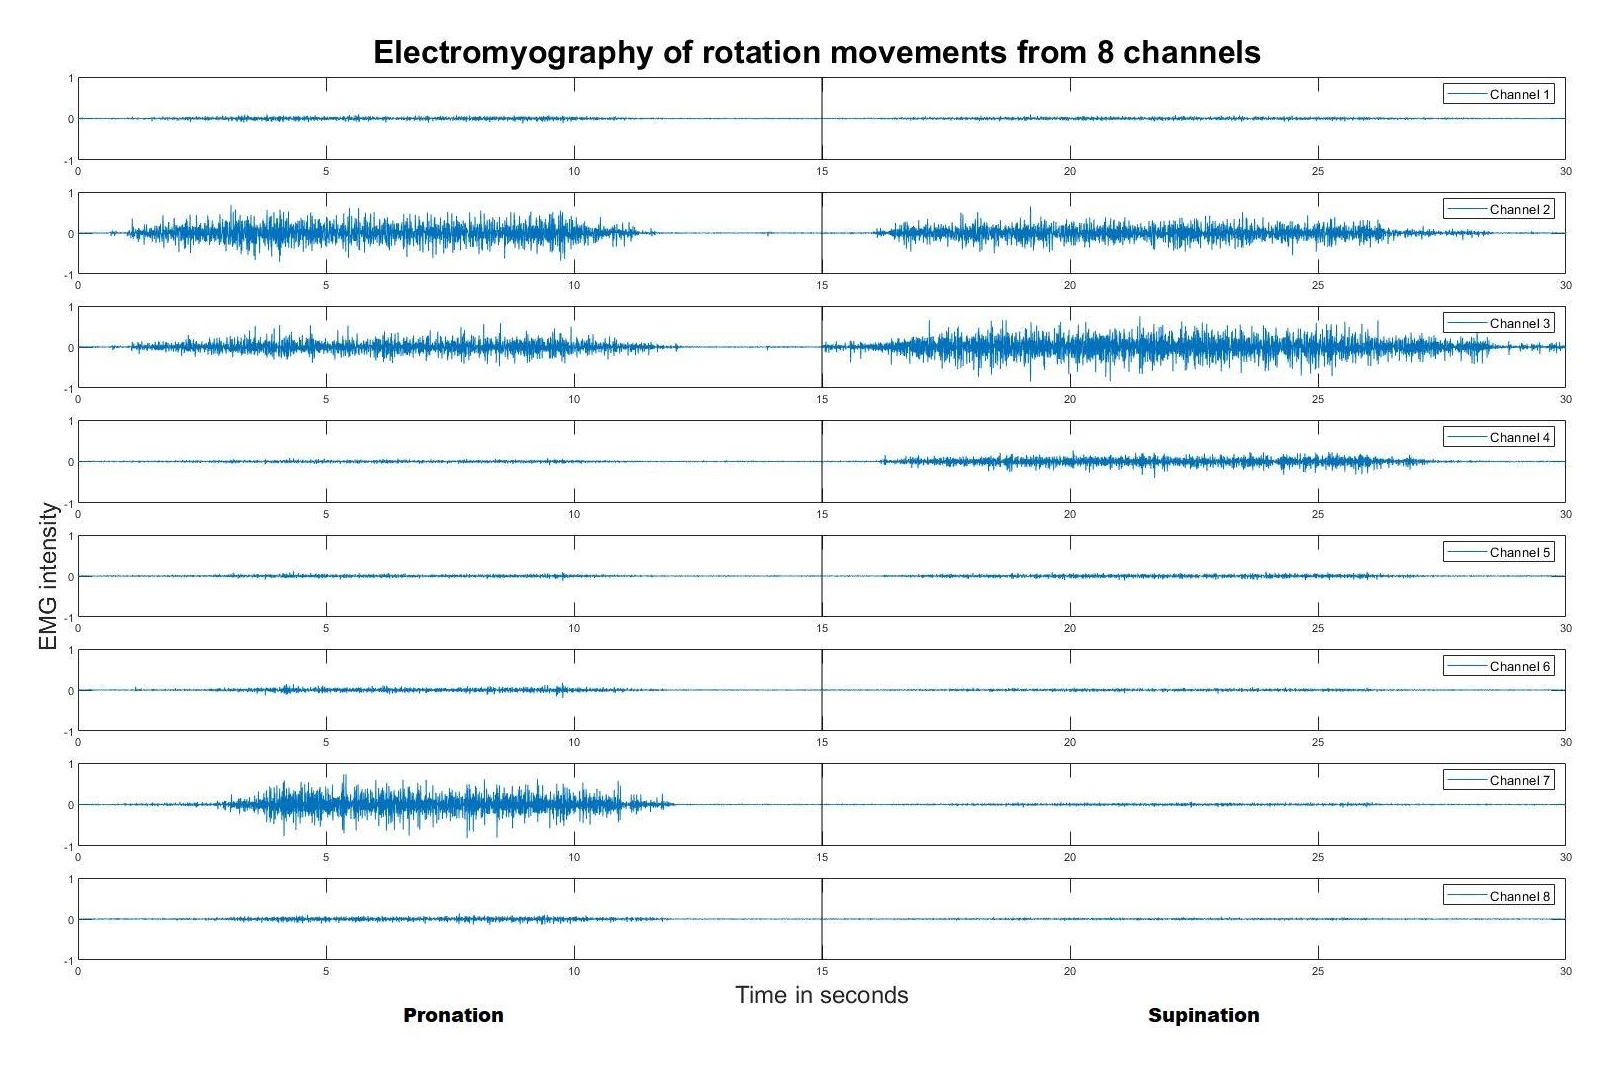
\includegraphics[width=1\textwidth]{figures/Emg_rot}  
	\caption{Illustration of an eight electrode channel surface EMG of the forearm during pronation (left side) and supination (right side) of the wrist. The recording was acquired using the Myo Armband, see \figref{fig:MYB}. The 4th channel was placed on the thickest part of the forearm centrally on the anterior side, when using a pronated arm as reference position, with the horizontal LED light faced laterally towards the wrist.}
	\label{fig:Emg_rot} 
\end{figure}

%surface and iemg emg             

\section{Prosthetic Control}

Throughout the development of myoelectric prosthetics, different control schemes have been derived, tested and some implemented in commercially available devices. Complexity and dexterity are dependent on the control system and before choosing a method one must form an overview of the opportunities each presents. The following section will present fundamental concepts of the main control methods. 
 
% Switch based control 
\subsection{Direct switch-based myoelectric control}
A Switch-based myoelectric is the conventional control method and is also known as on/off, crisp, binary or bang/bang control. \cite{Geethanjali2016}
Signal preprocessing is simple and the signal is usually only rectified and filtered. Various sub-control schemes exist, which are either based on the EMG-amplitude of one or two channels. The user is able to control one DoF (e.g. open/closed hand), recorded from one channel, by surpassing a lower amplitude threshold for open hand and a higher closed hand. Alternatively the EMG-signal can be recorded from two independent muscles (two channels) and if a threshold is exceeded in one, the prosthesis would move in a predetermined direction. An illustration of both one and two-channel control schemes can be seen in \figref{fig:Sw}. The actuation speed can be at a fixed speed or proportionally to the EMG amplitude. Multiple DoF's can be achieved by switching the DoF-mode by providing a quick mode-switch signal e.g. two quick contractions, or by physically pressing a switch on the prosthesis. \cite{Farina2014,Wurth2014}  The two channel direct switch-based control scheme can be found in the commercially available Michelangelo Hand \cite{Ottobuck2019}. \\  Switch-based is a simplistic, but slow  control approach. Furthermore, it quickly gets impractical and non-intuitive when increasing the number of DoF's to be replaced as the intended movement is unrelated to the acquisition site. Additionally, the methods relies on isolated muscle contractions, sensitivity might me decreased by channel cross-talk and muscle co-activation. \cite{Wurth2014}    
   
   
 \begin{figure}[H] 
 	\centering
 	\subfigure[One channel threshold control.]
 	{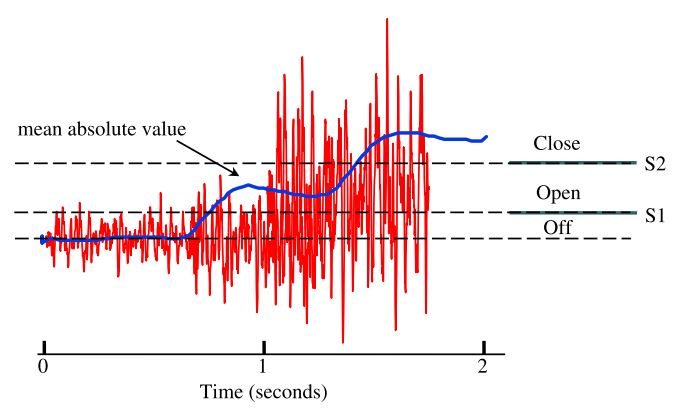
\includegraphics[width=.49\textwidth]{figures/Switch1}}
 	\subfigure[Two channel threshold control.]
 	{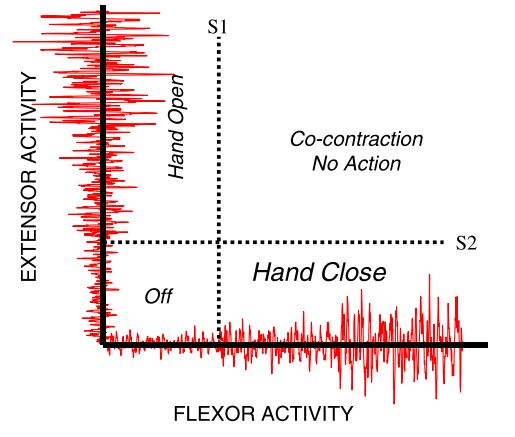
\includegraphics[width=.4\textwidth]{figures/Switch2}}  
 	\caption{Illustration of a direct one channel (a) and two channel (b) threshold control schemes using EMG amplitude to control open/close hand function. S denotes a threshold. Illustration taken from \cite{Parker2006}.}
 	\label{fig:Sw}
 \end{figure}  
   
   
%sequential 
\subsection{Sequential myoelectric control}

To overcome the disadvantages of direct switch-based control in slow and not intuitive control, alternative control strategies relying on algorithms have been derived. Such algorithms could utilize classification-based pattern recognition to predict the intended movement of the user. Often signal from several electrodes are captured. An assumption is that given a consistent movement task is performed the muscles will exhibit a unique activation pattern, and that features extracted from each signal for each movement type can be used to distinguish between different movement types. Hence, complex EMG-signal patterns can be assigned to discrete movement classes, thus also allowing for control of several DoF's.  \cite{Farina2014,Wurth2014}  \\
This approach is more intuitive as it does not demand the need for switching between DoF's, and lowering the amount of effort the user has to put in completing a task. A disadvantage of sequential control is lack of simultaneously controlling multiple DoF's at once allowing for a faster and more natural task execution. \cite{Farina2014}  

%Simultaneous
\subsection{Simultaneous myoelectric control}

Incorporating intuitiveness and naturalness in prosthetic control can be achieved through simultaneous control, where more than one DoF is controlled at a time. Pattern recognition methods predicting more than one movement type have been proposed, but naturalness through proportional actuation speed cannot be achieved independently for each DoF. Instead regression-based methods have been introduced. Compared to classification, which will output one class, trained regressors will continuously output the estimated value for each movement type. Choosing the two movement, which fit the regressors the best will provide simultaneous and proportional control. \cite{Hahne2014} 



	
\urlstyle{same}
\printbibliography\clearpage



\cleardoublepage
% BILAG
\begin{appendices}
\chapter{Appendices}

\end{appendices}


\end{document}
